Several previous authors have used the GEANT4 toolkit to simulate the light collection efficiency of their detector designs.
In PNNL 14283 the authors looked at a variety of different PMT placement and detectors designs to increase the light output of a detector in the Advanced Large-Area Plastic Scintillators (ALPS) project \cite{pnnl_14283}.
The authors found that for a \SI{127}{\cm} by \SI{57}{\cm} by \SI{5}{\cm} slab of BC-408 (a typical PVT based plastic scintillator) wrapped in a loose foil of 85\% reflectivity that the light output could be almost doubled by doubling the number of PMT's.
These results are summarized in \autoref{tab:PNNLLightCollectionEfficiency}. 
For this detector design the number of PMT's was set at two, 2 inch PMTs with the knowledge of adding additional PMTs will increase the light collection.
\begin{table}
  \centering
  \caption[PNNL Light Collection Efficiencies]{Light collection efficiencies of several detector designs simulated by PNNL\cite{pnnl_14283}. The detector is BC-408 (PVT based scintillator) of dimensions \SI{127}{\cm} x \SI{57.15}{\cm} x \SI{5.08}{\cm}.}
  \label{tab:PNNLLightCollectionEfficiency}
  \begin{tabular}{c|c c}
  \toprule
  & \multicolumn{2}{c}{Light Collection Efficiency} \\
  Number of PMTs  & 2-in PMT & 5-in PMT \\
  \midrule
  2 & 7.0\% & 18.8\% \\
  4 & 13.3\% & 30.7\ \\
  6 & 18.4\% & 40.2\% \\
  \bottomrule
  \end{tabular}
\end{table}

The choice of cladding around the light guide and detector is essential to optimize the number of optical photons collected.
The cladding material must be matched for the wavelength of the photons that are being transported as well as the index of refraction of the material, taking into account the bulk absorption of the material and specular or diffusive reflection as the boundaries.
A GEANT4 simulation was then completed of a PVT based scintillator, polystyrene loaded with 10\% \iso[6]{LiF} scintillator, and \iso[6]{LiF} loaded ZnS:Ag scintillator with claddings of air, mylar, and teflon.
The collection efficiencies are presented in \autoref{tab:CladStudy}.
It was then determined that Teflon tape would be the best material to ensure that the highest fraction of photons are collected.
\begin{table}
  \caption[Teflon, Mylar, and HDPE Cladding Light Collection Effect]{The effect of Teflon, mylar, and air cladding on the light collection of a scintillating slab. The simulation is \SI{100}{\um} thick slice of material \SI{2}{\m} long, \SI{30}{\cm} wide with a rectangular PMT on each end. The photons are born isotropically throughout the material. It should be noted that there is substantial self-absorption in ZnS:Ag, which results in a very small fraction of the photons collected. In practice, however, ZnS:Ag is bright enough that it out performs the other materials.}
  \label{tab:CladStudy}
  \begin{tabular}{p{3cm} m{3cm} m{3cm} m{3cm}}
  \toprule
  & Coating & Fraction of Photons Collected & Expected Number of Photons Collected \\
  \midrule 
  \multirow{3}{*}{EJ-200} & Teflon & 12\% & 1,200\\
  				      & Air &  14\% & 1,400\\
				      & Mylar & 9.6\% & 960\\
  \midrule 
  \multirow{3}{*}{PS LiF} & Teflon & 4.3\% & 86\\
  				      & Air & 4.5\% & 90\\
				      & Mylar & 4.0\% & 80\\
  \midrule 
  \multirow{3}{*}{EJ-426} & Teflon & 0.46\% &736\\
  				      & Air & 0.45\% & 720\\
				      & Mylar & 0.42\% & 672 \\
 \bottomrule				 	   				  
 \end{tabular}
\end{table}
In order to decrease the optical photon absorption a wavelength shifting bar was employed.
The effect of using a wavelength shifting bar instead of PMMA of a light guide is dramatic; a factor of almost 10 more photons are detected when the wavelength shifting bar is employed.
  \begin{table}
  \caption[Light Collection Increase with a WLS Bar]{Effect of a WLS on the light collection of a scintillating slab. The simulation is \SI{100}{\um} thick slice of material \SI{2}{\m} long, \SI{30}{\cm} wide with a rectangular PMT on each end.}
  \label{tab:WLSStudy}
  \begin{tabular}{p{4cm} m{3cm} m{3cm}}
  \toprule
  & \multicolumn{2}{c}{Precent Photons Detected} \\
  Detector Material & PMMA &  WLS \\
  \midrule
 EJ-200 & 0.68\%  & 12\% \\
 PS LiF & 0.14\% & 4.3\% \\
 EJ-426 & \num{1.3E-3}\% & \num{4.5E-3}\% \\
 \bottomrule
  \end{tabular}
\end{table}

A four layered detector design was then simulated with GEANT4 in order to determine the number of optical photons that were collected.
This design has the \SI{100}{\um}, 10\% loaded \iso[6]{LiF} films sandwiched between wavelength shifting (each \SI{5}{\mm} thick) with a single PMT at the top and bottom.
This design collects 8\% of the optical photons emitted; for a polystyrene film with an average light yield of 2,000 photons per neutron 400 would then hit the photocathode.
It is expected that this is enough photons to create a signal above the noise for a typical PMT, while an increased signal can be achieved by additional PMTs.
\begin{figure}
  \centering
	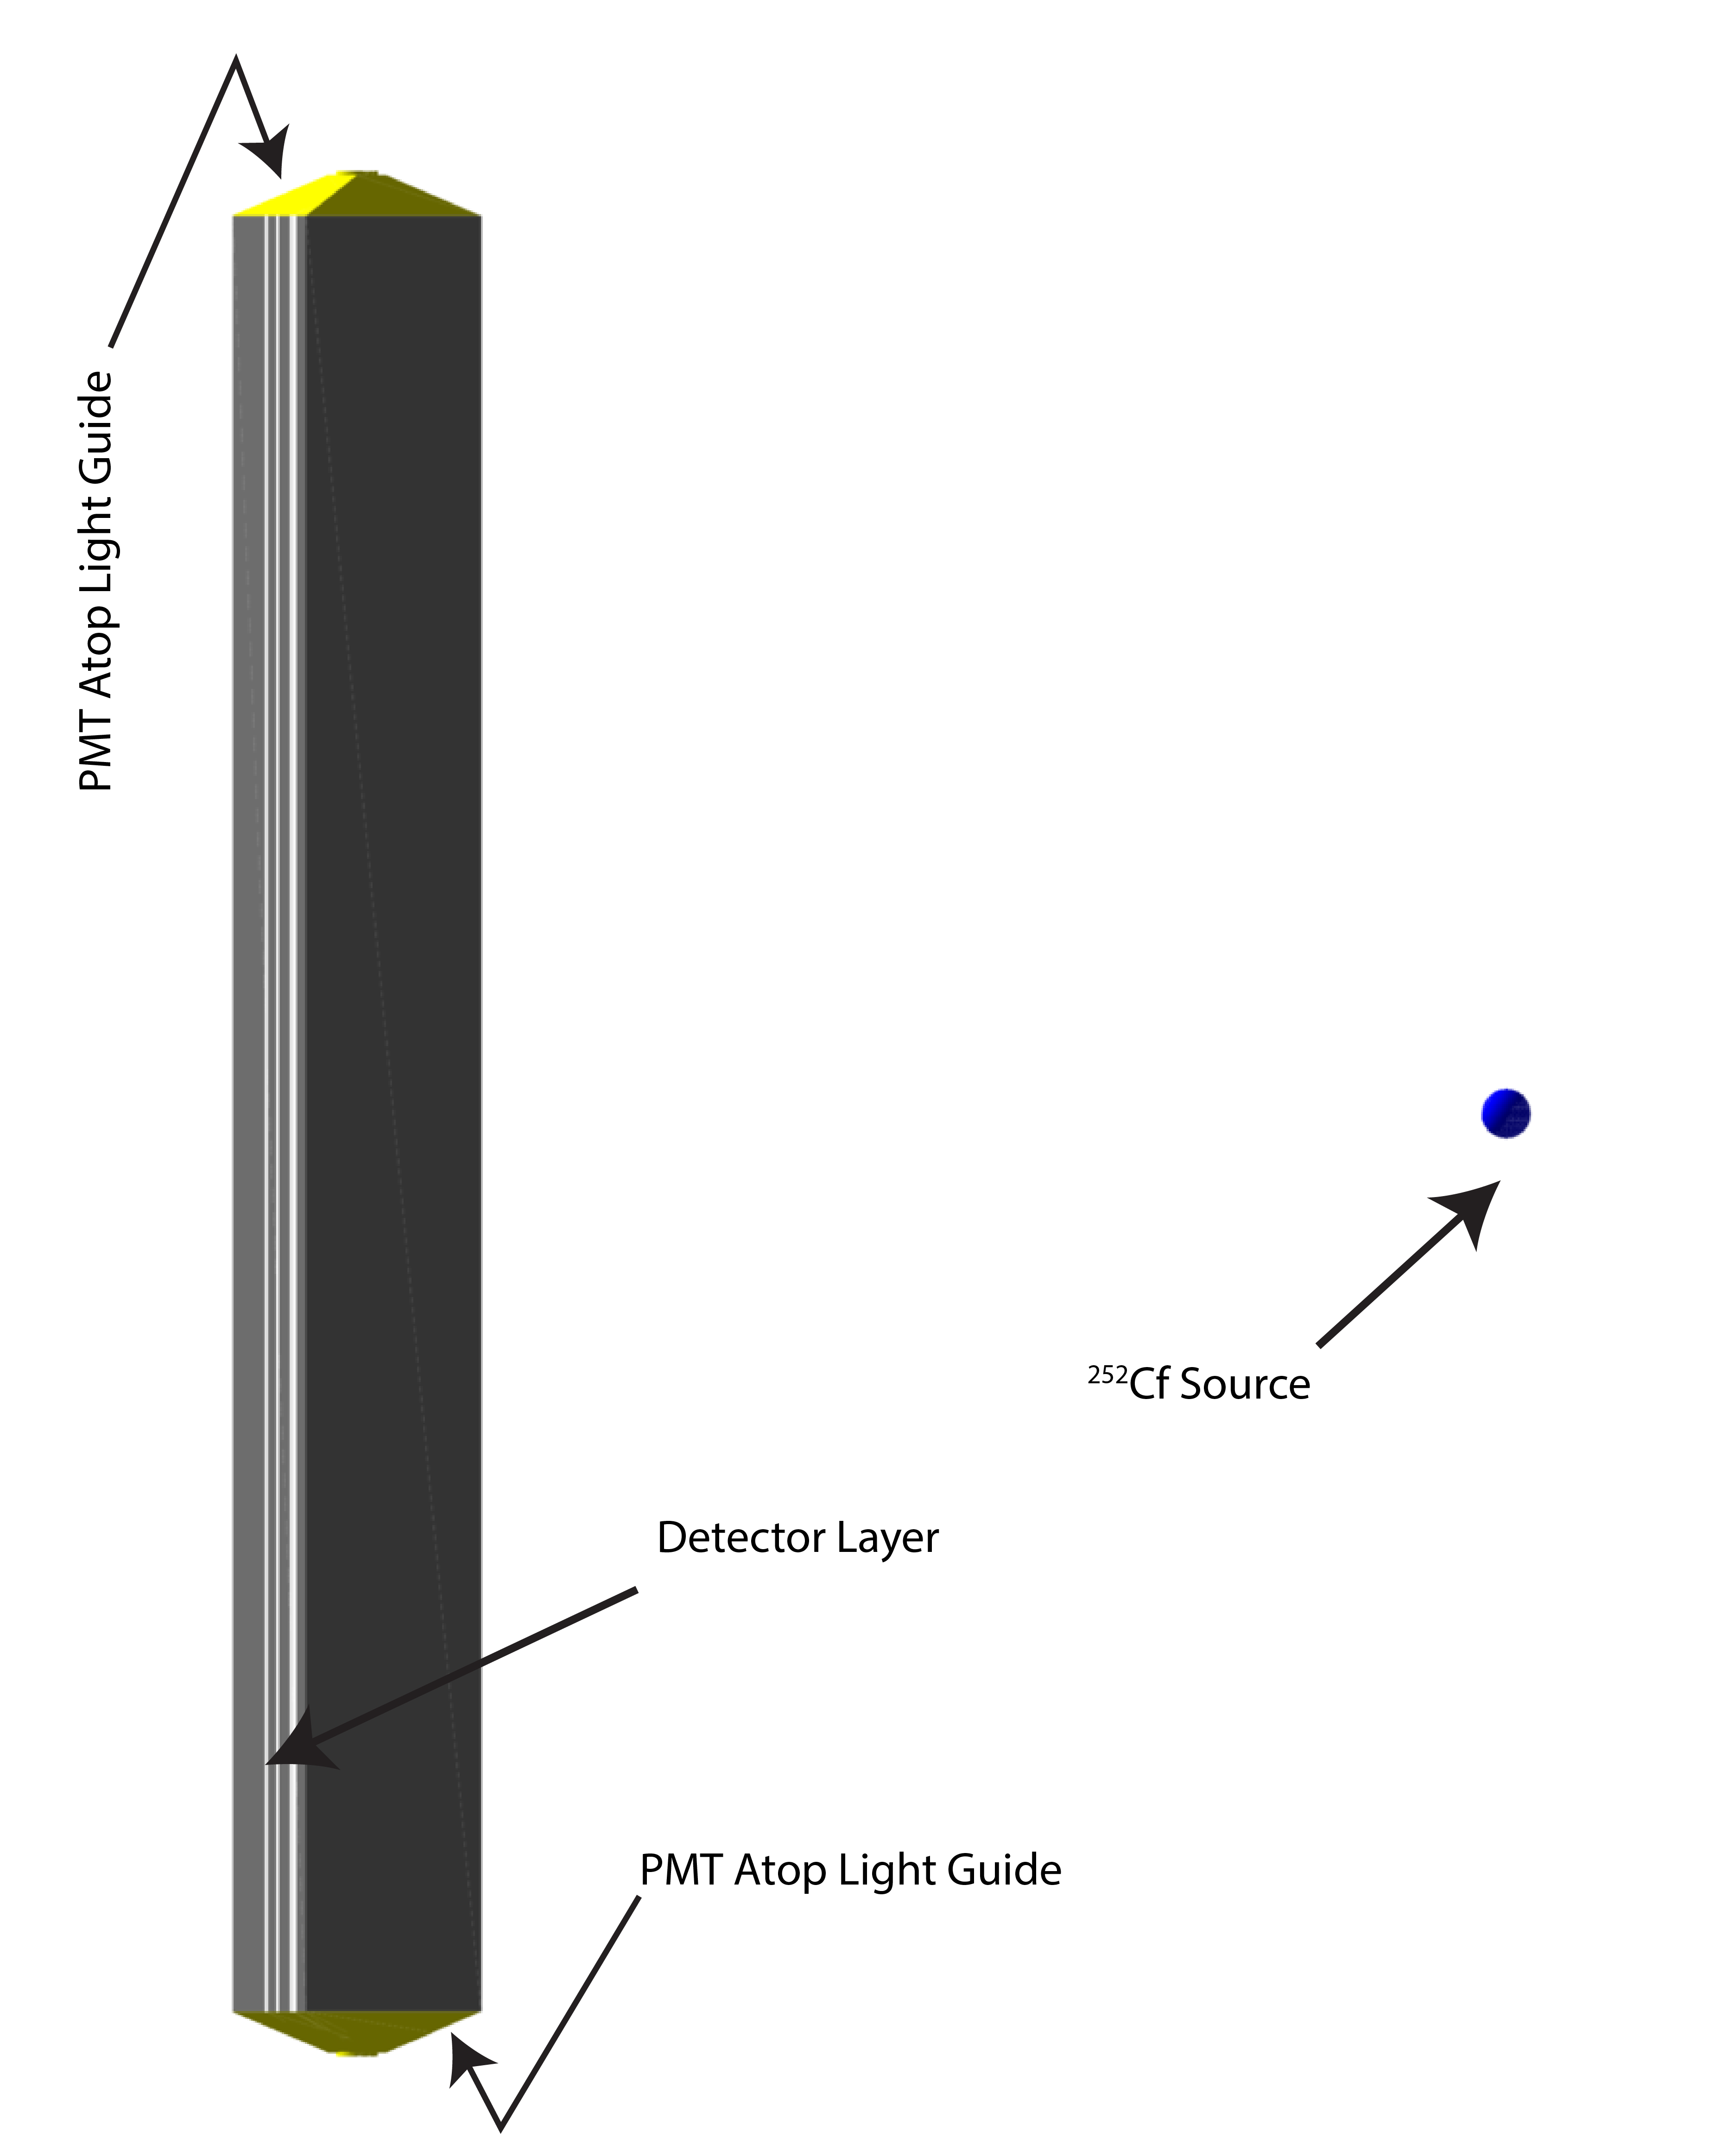
\includegraphics[width=\textwidth]{GEANT4AnnotatedGeo_RPM8SimGeo}
	  \caption[GEANT4 Simulated RPM8 Detector Design]{Simulated RPM8 with light transport in GEANT4. This design is capable of meeting all of the criteria set forth for radiation portal monitors.}
  \label{fig:G4RPM8Geo}
\end{figure}

